\PassOptionsToPackage{unicode=true}{hyperref} % options for packages loaded elsewhere
\PassOptionsToPackage{hyphens}{url}
%
\documentclass[12pt,,a4paper]{article}
\usepackage{lmodern}
\usepackage{amssymb,amsmath,mathtools,multirow}
\usepackage{float,hhline}
\usepackage{tikz}
\usepackage[tikz]{bclogo}
\usepackage{mathtools}
\usepackage{ifxetex,ifluatex}
\usepackage{fixltx2e} % provides \textsubscript
\ifnum 0\ifxetex 1\fi\ifluatex 1\fi=0 % if pdftex
  \usepackage[T1]{fontenc}
  \usepackage[utf8]{inputenc}
  \usepackage{textcomp} % provides euro and other symbols
\else % if luatex or xelatex
  \usepackage{unicode-math}
  \defaultfontfeatures{Ligatures=TeX,Scale=MatchLowercase}
\fi
% use upquote if available, for straight quotes in verbatim environments
\IfFileExists{upquote.sty}{\usepackage{upquote}}{}
% use microtype if available
\IfFileExists{microtype.sty}{%
\usepackage[]{microtype}
\UseMicrotypeSet[protrusion]{basicmath} % disable protrusion for tt fonts
}{}
\IfFileExists{parskip.sty}{%
\usepackage{parskip}
}{% else
\setlength{\parindent}{0pt}
\setlength{\parskip}{6pt plus 2pt minus 1pt}
}
\usepackage{hyperref}
\hypersetup{
            pdftitle={Performance of asymmetric filters for trend-cycle extraction, application to the COVID-19 crisis},
            pdfkeywords={trend-cycle extraction, asymmetric filters, R, seasonal adjustment},
            pdfborder={0 0 0},
            breaklinks=true}
\urlstyle{same}  % don't use monospace font for urls
\usepackage[true]{geometry}
\usepackage{longtable,booktabs}
% Fix footnotes in tables (requires footnote package)
\IfFileExists{footnote.sty}{\usepackage{footnote}\makesavenoteenv{longtable}}{}
\setlength{\emergencystretch}{3em}  % prevent overfull lines
\providecommand{\tightlist}{%
  %\setlength{\itemsep}{0pt}
  \setlength{\parskip}{0pt}
  }
\setcounter{secnumdepth}{5}
% Redefines (sub)paragraphs to behave more like sections
\ifx\paragraph\undefined\else
\let\oldparagraph\paragraph
\renewcommand{\paragraph}[1]{\oldparagraph{#1}\mbox{}}
\fi
\ifx\subparagraph\undefined\else
\let\oldsubparagraph\subparagraph
\renewcommand{\subparagraph}[1]{\oldsubparagraph{#1}\mbox{}}
\fi

% set default figure placement to htbp
\makeatletter
\def\fps@figure{htbp}
\makeatother

\usepackage{fancyhdr}

%\cfoot{ {\fontsize{8pt}{9.6pt}\selectfont 6\par}}

%% NO HEADING...
%%\fancyhead[RE]{\headreport}
%%\fancyhead[RO,LE]{\bfseries\thepage}
%%\fancyhead[LO]{\nouppercase{\rightmark}} %{\markright} %{\sectionmark}

\pagestyle{fancy}
\fancyhf{}

\usepackage{sectsty}
\usepackage{setspace}

\renewcommand{\headrulewidth}{0pt}
\setlength{\topsep}{0pt}\setlength{\parindent}{0pt}

\renewcommand{\arraystretch}{1.3}
\setcounter{tocdepth}{4}
\setcounter{secnumdepth}{4}


%% depths for Sections 
% 1) Section
% 1.1) SubSection
% 1.1.1) SubSubSection
% 1.1.1.1) Paragraph
\setcounter{tocdepth}{4}
\setcounter{secnumdepth}{4}

% depths for nested lists created by \begin{enumerate}
\usepackage{enumitem}
\setlistdepth{9}
\renewlist{enumerate}{enumerate}{9}
	\setlist[enumerate,1]{label=\arabic*)}
	\setlist[enumerate,2]{label=\alph*)}
	\setlist[enumerate,3]{label=(\roman*)}
	\setlist[enumerate,4]{label=(\arabic*)}
	\setlist[enumerate,5]{label=(\Alph*)}
	\setlist[enumerate,6]{label=(\Roman*)}
	\setlist[enumerate,7]{label=\arabic*}
	\setlist[enumerate,8]{label=\alph*}
	\setlist[enumerate,9]{label=\roman*}
\renewlist{itemize}{itemize}{9}
	\setlist[itemize]{label=$\cdot$}
	\setlist[itemize,1]{label=\textbullet}
	\setlist[itemize,2]{label=$\circ$}
	\setlist[itemize,3]{label=$\ast$}
	\setlist[itemize,4]{label=$\dagger$}
	\setlist[itemize,5]{label=$\triangleright$}
	\setlist[itemize,6]{label=$\bigstar$}
	\setlist[itemize,7]{label=$\blacklozenge$}
	\setlist[itemize,8]{label=$\prime$}

% that's for generating directly PDF documents using pdfLaTex instead of LaTex alone
\newif\ifpdf\ifx\pdfoutput\undefined\pdffalse\else\pdfoutput=1\pdftrue\fi
\newcommand{\pdfgraphics}{\ifpdf\DeclareGraphicsExtensions{.pdf,.png,.tif,.jpg}\else\fi}


\usepackage{amsmath}
\usepackage{latexsym}
\usepackage{amsfonts}
\usepackage[normalem]{ulem}
\usepackage{array}
\usepackage{amssymb}

\ifpdf
\usepackage[pdftex]{graphicx}
\else
\usepackage{graphicx}
\fi

\usepackage{float}
%\usepackage{subfloat}
\usepackage{subfig}
% \usepackage[list=true]{subcaption} % cannot be used conjointly with subfig
\usepackage{wrapfig}
\usepackage{wasysym}
%\usepackage[svgnames,table,rgb]{xcolor}
\usepackage{longtable} % long tabulars
\usepackage{adjustbox}
\usepackage{alltt} % verbatim 
\usepackage{changepage}
\usepackage{hhline}
\usepackage{multicol}
\usepackage{tabto}
\usepackage{multirow}
%\usepackage{ragged2e}
%\usepackage{makecell}
%\usepackage[toc,page]{appendix}

% usually not necessary if you include figures as png/jpg...
\usepackage{pgfplots}
\usepackage{tikz}
\usetikzlibrary{arrows,backgrounds,snakes}

\urlstyle{same}


 %% HEADER
\title{
\vspace{-5ex}
\thetitle
\vspace{-2ex}
}
\author{
\theauthors
\vspace{-5ex}
}
\date{}

\newcommand*{\doi}[1]{DOI: \href{https://doi.org/\detokenize{#1}}{\detokenize{#1}}} 
\newcommand*{\arxiv}[1]{arXiv: \href{https://arxiv.org/abs/\detokenize{#1}}{\detokenize{#1}}} 

% Ajout AQLT
\usepackage{fontawesome5}
\usepackage{stmaryrd}
\DeclareMathOperator{\e}{e}
\usepackage{animate, dsfont, here, xspace}

\ifnum 0\ifxetex 1\fi\ifluatex 1\fi=0 % if pdftex
  \usepackage[shorthands=off,main=]{babel}
\else
  % load polyglossia as late as possible as it *could* call bidi if RTL lang (e.g. Hebrew or Arabic)
  \usepackage{polyglossia}
  \setmainlanguage[]{}
\fi
\usepackage[numbers]{natbib}
\bibliographystyle{unsrtnat}

\title{Performance of asymmetric filters for trend-cycle extraction, application to the COVID-19 crisis}
\date{}



\DeclareMathOperator{\Cov}{Cov}
\newcommand{\E}[1]{\mathbb{E}\left[ #1 \right]}
\newcommand{\V}[1]{\mathbb{V}\left[ #1 \right]}
\newcommand{\cov}[2]{\Cov\left( #1\,,\,#2 \right)}

\begin{document}
\maketitle

\hypertarget{introduction}{%
\section{Introduction}\label{introduction}}

With the COVID-19 crisis, one of the major questions on the economy was when it will collapse and when it will recover.
It illustrates that business cycle analysis, and in particular the early detection of turning points in a series, is a major topic in the analysis of economic outlook.

Moving averages, or linear filters, are ubiquitous in business cycle extraction and seasonal adjustment methods.
For example, the X-12ARIMA seasonal adjustment method uses Henderson moving averages and composite moving averages to estimate the main components of a time series, while TRAMO-SEATS uses Wiener-Kolmogorov filters.
Symmetric filters are applied to the center of the series, but when it comes to estimate the most recent points, all of these methods must rely on asymmetric filters.
For example, even if X-12ARIMA or TRAMO-SEATS apply symmetrical averages to the forecasts obtained from an ARIMA model of the series, in reality it consists in applying asymmetric filters at the end of the series, because the predicted values are linear combinations of past values.

If the classic asymmetric moving averages have good properties regarding the future revisions induced by the process, they create phase shifts that impact the real-time estimation of turning points, introducing time delay in the detection.

This report aims to describe and compare the recent approaches around trend-cycle extraction and asymmetric filters, applying them to the COVID-19 economic crisis.
All the methods being implemented in the \faIcon{r-project} package \texttt{rjdfilters}\footnote{Available at \url{https://github.com/palatej/rjdfilters}.}, the results can be easily reproduced.

\hypertarget{methods}{%
\section{Methods}\label{methods}}

Let \(p\) et \(q\) two integers, a moving average \(M_\theta\) is defined by a set of coefficients \(\theta=(\theta_{-p},\dots,\theta_{q})'\) such as for all time series \(X_t\):
\[
M_\theta(X_t)=\sum_{k=-p}^{+q}\theta_kX_{t+k}
\]
Therefore, applying a moving average \(M_\theta\) to the time series \(X_t\) consists in applying a rolling weighted mean to a times series: for each date it computes a weighted mean of \(p\) past points and \(q\) future points.

For trend-cycle extraction, the moving averages usually used are \emph{symmetric}: \(p=q\) and \(\forall k:\:\theta_{-k} = \theta_k\).
The \textbf{Henderson filter} is a filter widely used: it's for example the filter used in the seasonal adjustment algorithm X-12ARIMA.

When it comes to the estimates of the most recent points, the \(q\) future points are not available.
The filters that are used are called asymmetric filters because \(q\leq p\): for \(q=0\), a real-time estimation is done.

Applying a moving average to a harmonic times series \(y_t=\e^{-i\omega t}\) can be written as \(M_{\theta_0}y_t=G_\theta(\omega)\e^{-i\Phi_\theta(\omega)}y_t\). It affects the input time series it in in two different ways:

\begin{itemize}
\item
  by multiplying it by an amplitude coefficient determined by the gain function \(G_{\theta}\left(\omega\right)\);
\item
  by ``shifting'' it in time by the time shift function \(\Phi_\theta(\omega)/\omega\), which directly affects the detection of turning points.
\end{itemize}

See figure \ref{fig:exgainPhase} for an example.

\begin{figure}[!ht]
\pgfplotsset{width=\textwidth,height=6cm,every axis legend/.append style={font=\footnotesize,
  at={(0.5,-0.1)},
  anchor=north}
    }
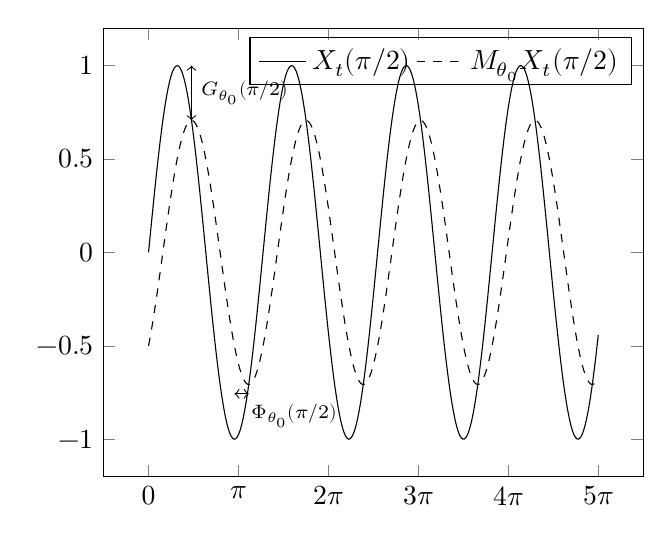
\begin{tikzpicture}
\begin{axis}[
legend columns=2,
legend style = {fill=none , fill opacity=0, draw opacity=1,text opacity=1},
xtick={0,3.14159,...,15.70795},
xticklabels={0,$\pi$,$2\pi$,$3\pi$,$4\pi$,$5\pi$} 
]
\addplot[domain=0:5*pi,smooth,samples=300]    plot (\x,{sin(\x * (pi/2) r)});
\addlegendentry{$X_t(\pi/2)$}
\addplot[domain=0:5*pi,smooth,samples=300, dashed]    
  plot (\x,{1/2*sin(\x* pi/2 r )+1/2*sin((\x -1) * pi/2 r)});
\addlegendentry{$M_{\theta_0}X_t(\pi/2)$}
\draw[<->](axis cs: 1.5,1)--(axis cs: 1.5,0.7071068)
  node[pos=0.5, right]{\scriptsize $G_{\theta_0}(\pi/2)$};
\draw[<->] (axis cs: 3, -0.70710680-0.05)--(axis cs: 3.5,-0.7071068-0.05) 
  node[pos=0.5, below right]{\scriptsize $\Phi_{\theta_0}(\pi/2)$};
\end{axis}
\end{tikzpicture}
\caption{Smoothing of the time series $y_t=\sin(\omega t)$ by the moving average $M_{\theta_0}y_t=\frac{1}{2}y_{t-1}+\frac{1}{2}y_{t}$ for $\omega=\pi/2$.}\label{fig:exgainPhase}
\end{figure}

Whereas symmetric filters do not create phase-shift, asymmetric filters do.
The different methods used to build asymmetric filters make a tradeoff between minimizing the phase-shift and minimizing the revisions to the symmetric filter.
Here we consider three recent approaches to build asymmetric filters:

\begin{itemize}
\item
  The one developed by \citet{proietti2008} that consists in locally approximated the trend by a polynomial trend.
  In this paper, three asymmetric filters are considered:

  \begin{itemize}
  \item
    The direct asymmetric filter (DAF): it's the filter directly obtained by estimating a local polynomial of degree 3 on the \(p+q+1\) observations.
  \item
    Linear-Constant (LC) filter: it's computed by assuming that trend of the input time series is linear and imposing that the asymmetric filter preserves constant trends.
  \item
    Quadratic-Linear (QL) filter: it's computed by assuming that trend of the input time series is quadratic and imposing that the asymmetric filter preserves linear trends.
  \end{itemize}
\item
  \citet{ch15HBSA} defined a general approach to derive linear filters, minimizing a weighted sum of three criteria subject to some constraints (usually polynomial preservation).
  The three criteria are: the fidelity (the variance reduction ratio of the filter), the smoothness (measures the flexibility of the coefficient curve of a filter and the smoothness of the trend) and the timeliness (measures the phase shift between input and output series for specific frequencies).\\
  For simplicity, in this paper we only retain an extreme filter than minimizes the phase shift by (putting a large weight to the timeliness) and that preserves linear trends, as defined by \citet{ch15HBSA}.
  This filter will be defined as the ``FST'' filter.
\item
  \citet{dagumbianconcini2008} developed a general approach to derive linear filters based on Reproducing Kernel Hilbert Space (RKHS) methodology.
  The weight of the filters depends on a time-invariant global bandwidth parameter that can be chosen by optimization of some criteria.
  We defined as \(b_{q,\phi}\) filter the one obtained with the bandwidth that produce asymmetric filters that minimize the phase shift.
\end{itemize}

\hypertarget{results}{%
\section{Results}\label{results}}

The figure \ref{fig:ipi} compares the different asymmetric filters applying them to the seasonally adjusted series of French industrial production index of the manufacturing industry\footnote{This series is produced by the INSEE, the French National Statistical Office, and is available at \url{https://bdm.insee.fr/series/sdmx/data/SERIES_BDM/010537946}.}.
The French industrial production is strongly impact by the COVID-19 economic crisis, in particular due to the mandatory lockdown of the population from March 17th to May 11th.

\begin{figure}[!ht]
\animategraphics[autoplay,loop,width=0.99\textwidth,controls]{2}{img/illustrationfr_}{1}{5}
\caption{Application of asymmetric filters to the French industrial production index (IPI) of manufacturing industry.}\label{fig:ipi}\footnotesize
\emph{Note: The symmetric trend is the one computed by a symmetric 13-terms Henderson filter.}

\emph{To see the animation, the PDF must be open with Acrobat Reader, KDE Okular, PDF-XChange or Foxit Reader.
Otherwise you will only be able to see the results for the DAF filter.}
\end{figure}

In this example, we can notice that the estimates of DAF, QL and FST filters have much more variability than the others: the real-time (\(q=0\)) trend-cycle estimates of April and May 2020 being very low.
Therefore, the real-time estimates are highly revised for those methods.

LC and \(b_{q,\phi}\) filters produce much smoother estimates.
However, we can expect more bias for those methods since the asymmetric filters only preserve constant trends, and so they distort the trend around turning points.

Except the DAF filter, all the methods detect an upturn in May 2020 and produce similar results when more than two future points are available (\(q\geq 2\)).
Besides, the estimates are much closer to the estimates of the symmetric filter (when it can be computed) than the DAF estimates.
Consequently, the DAF estimates will certainly be more revised than the other ones.

Those results should be taken with precaution: the series used is seasonally adjusted and in this process the last estimates are made with an asymmetric filter.
Moreover, during the COVID crisis the last points are considered as outliers and are corrected for the decomposition process.
Therefore, this study should be extend to see the impact of the different asymmetric filters also on the seasonally adjusted series.

\hypertarget{conclusions}{%
\section{Conclusions}\label{conclusions}}

To sum up, the different methods can lead to very different trend-cycle estimates.
However, all the methods produce better results than the direct asymmetric filters.
Consequently, there is no need to seek to preserve polynomial trends of degree more than one to build asymmetric filters.

Only focusing on the timeliness criteria (FST filter), highly increases the variance of the estimates: a tradeoff with other criteria must be maid.

Finally, for the last-points estimates of the trend-cycle component, the choice of the asymmetric filter should also take into account an economic analysis to decide which estimates are economically plausible.

This study could, for example, be extended in two ways.
Firstly studying the impact of the different methods on the seasonal adjustment process.
Secondly studying the impact of atypical points on the estimates and exploring new kinds of asymmetric filters based on robust methods (like robust local regressions).

\renewcommand\refname{References}
\bibliography{biblio.bib}

\end{document}
